\chapter{Introduction}

\section{Abstract}
\begin{figure}[htp]
\begin{center}
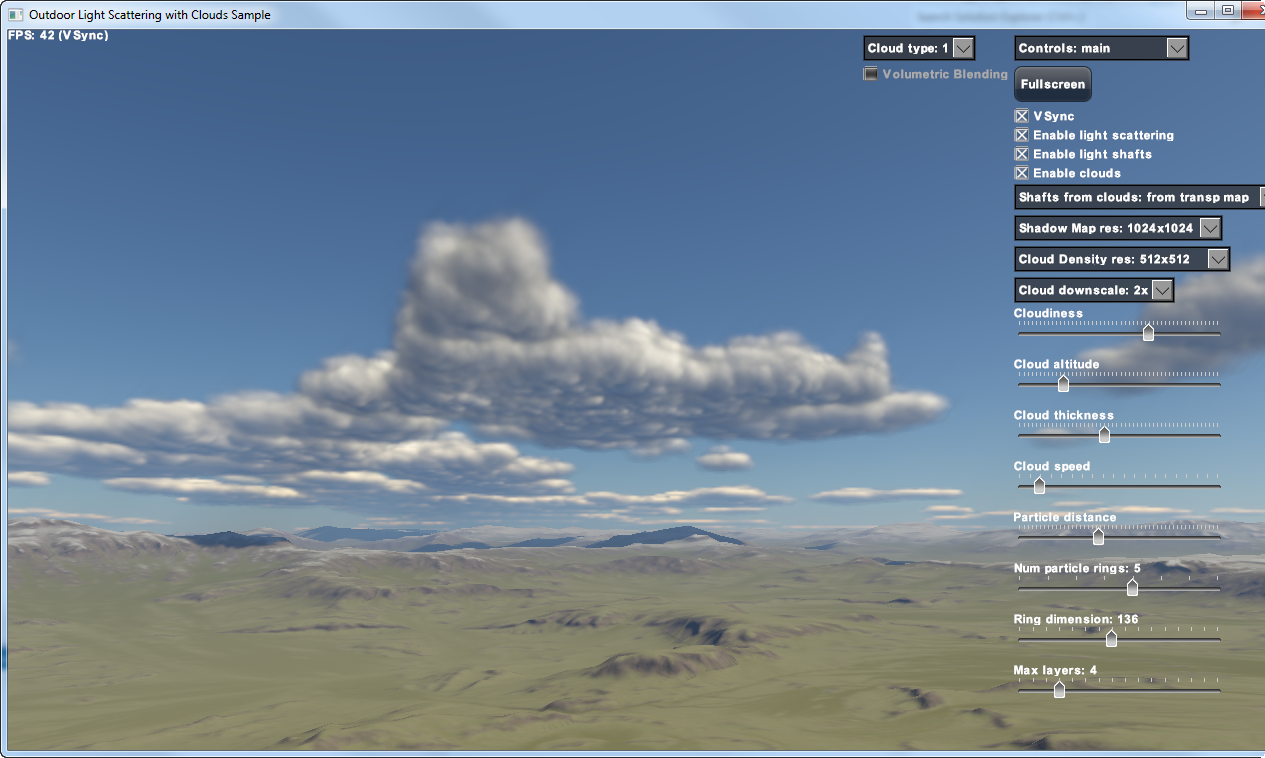
\includegraphics[scale=0.3]{images/overview.png}
\caption{Overview}
\label{f0}
\end{center}
\end{figure}

In the paper, the author introduced a new method for rendering realistic cumulus clouds in real time. The basic steps include:
\begin{enumerate}
\item Pre-computing optical depth.
\item Pre-computing scattering.
\item Generating a real-time lighting model from the above two steps.
\item Volume-aware blending the particles.
\item Controlling the level of details.
\end{enumerate}
He also explained the mathematical background to solve the problem. The paper is interesting, but hard to understand for a person not in the field. I'm writing this review to make the author's idea easier to be understood. I will also supplement to some uncertain explanation from the author with my personal thoughts.